\chapter{Deprecated vs.\ Corrected Optics: A Full Comparison}
\label{ch:deprecated_vs_corrected}

Chapter~\ref{ch:physics_audit} presented the before/after optimum-aperture table for a
subset of myopia levels. This chapter re-derives that comparison directly, on the full
$15\times8$ grid, by running the deprecated \texttt{stage2/} pipeline through the
identical sweep machinery used for every corrected-optics result in this report ---
isolated so that it can never contaminate any other chapter's numbers
(Appendix~\ref{app:software}).

\begin{figure}[htbp]
\centering
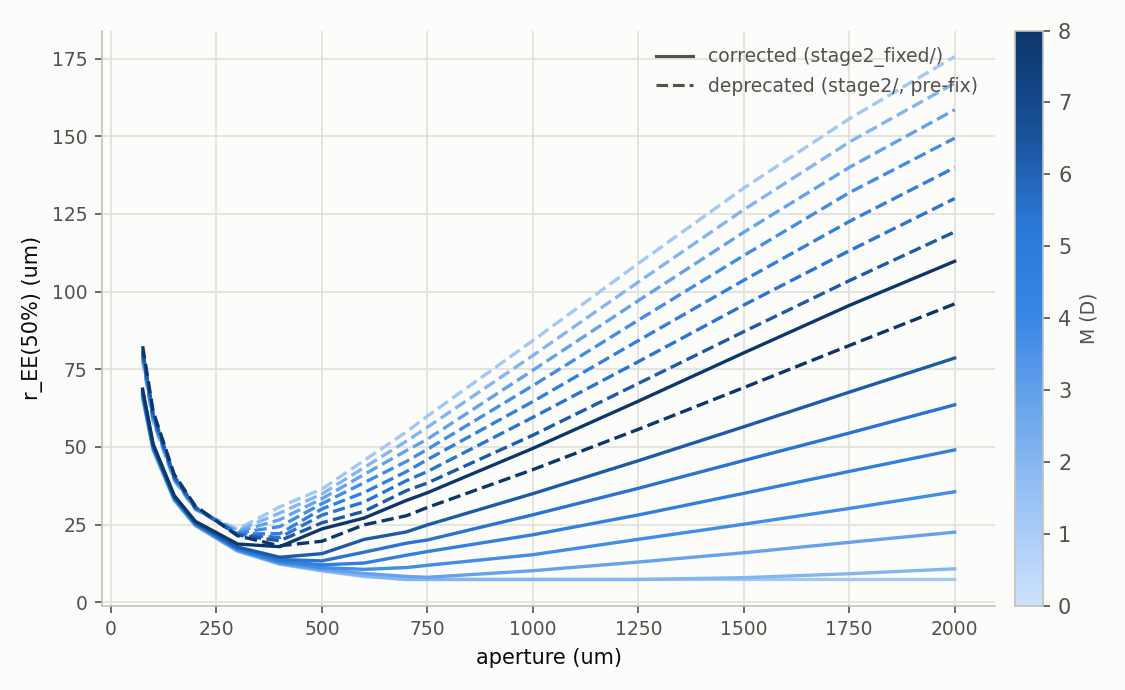
\includegraphics[width=0.85\textwidth]{figures/fig_deprecated_vs_corrected_overlay.png}
\caption{$r_{EE}(50\%)$ vs.\ aperture: corrected optics (solid) vs.\ deprecated pre-fix optics (dashed), one color per myopia level.}
\label{fig:deprecated-vs-corrected}
\end{figure}

{\small
\begin{longtable}{rrrr}
\caption{Optimal aperture, corrected vs. deprecated optics, full grid.}\label{tab:dep-vs-corr-full}\\
\toprule
M (D) & corrected optimum (um) & deprecated optimum (um) & change (\%) \\
\midrule
\endfirsthead
\multicolumn{4}{c}{\tablename\ \thetable\ -- continued}\\
\toprule
M (D) & corrected optimum (um) & deprecated optimum (um) & change (\%) \\
\midrule
\endhead
\bottomrule
\endfoot
0.00 & 700.00 & 300.00 & 133.33 \\
1.00 & 700.00 & 300.00 & 133.33 \\
2.00 & 750.00 & 300.00 & 150.00 \\
3.00 & 600.00 & 300.00 & 100.00 \\
4.00 & 500.00 & 300.00 & 66.67 \\
5.00 & 500.00 & 400.00 & 25.00 \\
6.00 & 400.00 & 400.00 & 0.00 \\
8.00 & 400.00 & 400.00 & 0.00 \\
\end{longtable}
}

The deprecated pipeline reports \emph{uniformly higher} blur radii than the corrected
one at every tested $(a_{hole}, M)$ combination --- consistent with
Chapter~\ref{ch:physics_audit}'s derivation that the bug under-applies the eye lens's
converging power, leaving every point somewhat out of focus relative to where the
corrected pipeline actually places the true focal plane. One further, non-obvious
consequence worth stating plainly: because the deprecated pipeline's blur is uniformly
larger, its retinal spots are less tightly focused, and \textbf{the deprecated pipeline
never exhibits the grid-resolution saturation artifact} of
Chapter~\ref{ch:percentile} at any myopia level tested here --- its own optimum-vs-$M$
table shows no tied minima at all, a coherent, physically sensible side effect of the
bug making every point blurrier rather than an inconsistency in the saturation
diagnosis itself.

\section{Does the fix's impact depend on which percentile is optimized?}

Chapter~\ref{ch:physics_audit}'s headline table used $r_{EE}(50\%)$ only. Repeating
the same corrected-vs-deprecated optimum-aperture comparison at this same spot for
$r_{EE}(70\%)$, $r_{EE}(80\%)$, and $r_{EE}(90\%)$ gives
Figure~\ref{fig:dvc-all-percentiles} and Table~\ref{tab:dvc-all-percentiles}.

\begin{figure}[htbp]
\centering
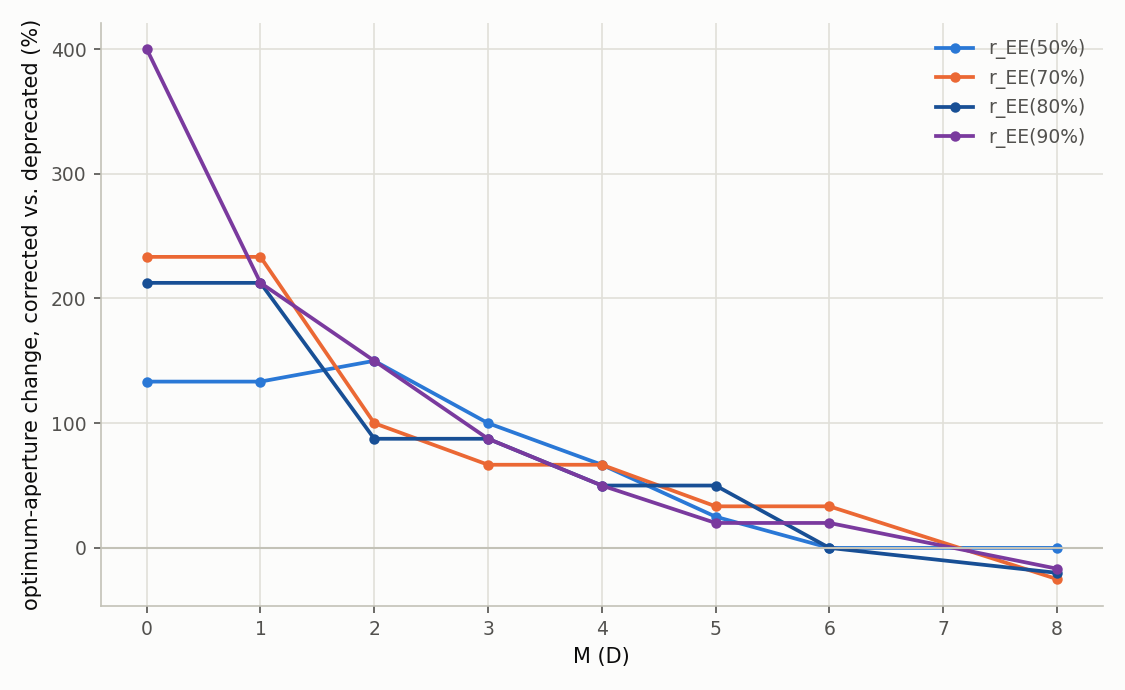
\includegraphics[width=0.85\textwidth]{figures/fig_deprecated_vs_corrected_all_percentiles.png}
\caption{Optimum-aperture change, corrected vs.\ deprecated optics, all four blur percentiles.}
\label{fig:dvc-all-percentiles}
\end{figure}

{\small
\begin{longtable}{rrrrr}
\caption{Optimal-aperture change, corrected vs. deprecated optics (\%), all four percentiles.}\label{tab:dvc-all-percentiles}\\
\toprule
M (D) & r\_EE(50\%) & r\_EE(70\%) & r\_EE(80\%) & r\_EE(90\%) \\
\midrule
\endfirsthead
\multicolumn{5}{c}{\tablename\ \thetable\ -- continued}\\
\toprule
M (D) & r\_EE(50\%) & r\_EE(70\%) & r\_EE(80\%) & r\_EE(90\%) \\
\midrule
\endhead
\bottomrule
\endfoot
0.0 & 133.3 & 233.3 & 212.5 & 400.0 \\
1.0 & 133.3 & 233.3 & 212.5 & 212.5 \\
2.0 & 150.0 & 100.0 & 87.5 & 150.0 \\
3.0 & 100.0 & 66.7 & 87.5 & 87.5 \\
4.0 & 66.7 & 66.7 & 50.0 & 50.0 \\
5.0 & 25.0 & 33.3 & 50.0 & 20.0 \\
6.0 & 0.0 & 33.3 & 0.0 & 20.0 \\
8.0 & 0.0 & -25.0 & -20.0 & -16.7 \\
\end{longtable}
}

The qualitative pattern from Chapter~\ref{ch:physics_audit} --- a large change at low
myopia collapsing toward $0\%$ by $M=6$--$8\,$D --- holds at every percentile, not
only $r_{EE}(50\%)$: the bug's absolute focal-shift error is independent of $M$, so it
dominates the (small) true defocus budget at low $M$ regardless of which blur
percentile measures it, and becomes proportionally negligible at high $M$ for the
same reason across all four. \textbf{Read the $M=0$--$1$ columns for
$r_{EE}(70\%)$/$r_{EE}(80\%)$ with the same caveat as Chapter~\ref{ch:percentile}}:
the corrected-optics side of that percentage change is, at those two myopia levels
specifically, drawn from a saturated (tied, non-unique) optimum, so the exact
percentage shown there is partly an artifact of which tied aperture happened to be
selected, not a fully clean measurement --- the $M\ge2$ columns are unaffected and
trustworthy.
